%!TEX root = origin_elements_lecture_notes.tex

\chapter{Short-lived Radionuclides in the Solar System}

In Chapter~\ref{ch:solar_system_abundances}, the solar abundances as measured in meteorites and in the Sun were discussed. Through the rest of this lecture, we then tried to explain how elements in the Milky Way formed, up to the point where the solar abundances can actually be explained. Finally, in the last chapter we discussed \ac{gce} models and how they try to recreate what we observe. 

In addition to stable nuclides, the Solar System also contained \acfp{slr} when it was formed. These \acp{slr} were incorporated into the first solids that formed and their record can still be deciphered by analyzing meteorites. While stable nuclides built up over the lifetime of the galaxy and thus require detailed \ac{gce} models to derive their formation and evolution, \acp{slr} must have formed and been injected into the solar nebula and / or the molecular cloud just prior to condensation of the first solids. 


\section{Observations}

It has been shown that the Solar System started with a canonical \ex{26}Al/\ex{27}Al ratio of $5\times10^{-5}$ \citep{jacobsen08}. Aluminum-26 is \iac{slr} with a half-life of $7.17\times10^{5}$\,a and decays to the stable \ex{26}Mg. This \ac{slr} must have been supplied to the solar nebula shortly before the collapse of the molecular cloud and the subsequent formation of the first solids. Let us first derive how to detect the presence of the long-decayed \ex{26}Al in meteoritic material. This technique, once established, can then easily be adopted to other \acp{slr}. 

\subsection{Isochrons Measurements}

\acp{slr} in meteorites can only be detected by analyzing their daughter products, since the original \ac{slr} has long decayed since it was incorporated 4.567\,Ga ago. Here, we will first discuss the determination of the initial \ex{26}Al of a given meteorite. This isotope has the additional advantage of being distributed homogeneously throughout the solar nebula, which allows us to use \ex{26}Al-\ex{26}Mg systematics in meteorites to compare the samples' relative ages. In an aluminum magnesium three-isotope plot, the constituents of a given sample will plot on a so-called isochron. This isochron describes a line and shows that all samples have a common age with respect to the \ac{slr} in question.

\begin{figure}[tb]
    \centering
    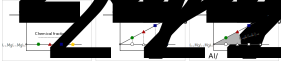
\includegraphics[width=\textwidth]{graphics/solar_system_slrs/al26_isochron}
    \caption{Schematic representation to show how an isochron develops over time in different minerals within a given meteorite.}
    \label{fig:solar_system_slrs:al26_isochron}
\end{figure}
Figure~\ref{fig:solar_system_slrs:al26_isochron} shows a schematic of the formation of an isochron. The left panel shows the aluminum and magnesium isotopic composition of various minerals a meteorite is composed of. The vertical axis hereby defines the \ex{26}Mg/\ex{24}Mg isotope ratio that is incorporated into the sample at time zero, i.e., when the sample condensed. Assuming a homogeneous solar nebula, all samples should plot at the same initial \ex{26}Mg/\ex{24}Mg ratio. The horizontal axis on the other hand shows the \ex{27}Al/\ex{24}Mg ratio, which is equivalent to the chemical composition of the constituents. Different minerals show different affinities to the incorporation of aluminum and magnesium into their matrix and therefore, these minerals ideally show a wide range of different \ex{27}Al/\ex{24}Mg compositions. While aluminum today only consists of \ex{27}Al, some radioactive \ex{26}Al was present in the early Solar System. Chemically, \ex{26}Al behaves in the same way as \ex{27}Al and therefore gets incorporated into the individual phases. The middle panel in Figure~\ref{fig:solar_system_slrs:al26_isochron} shows that over time, \ex{26}Al decays to \ex{26}Mg, which therefore raises \ex{26}Mg/\ex{24}Mg isotope ratio in the given mineral. Today, the amount of aluminum that was originally incorporated into each mineral correlates linearly with the \ex{26}Mg/\ex{24}Mg measured in a given sample. If multiple constituents of a given meteorite that show varying \ex{27}Al/\ex{24}Mg ratios are analyzed, the slope of the linear correlation determines the initial \ex{26}Al/\ex{27}Al of the sample. This is shown in the rightmost panel of Figure~\ref{fig:solar_system_slrs:al26_isochron}. The intercept of this linear correlation furthermore represents the original \ex{26}Mg/\ex{24}Mg that the sample started out with, i.e., the composition without any \ex{26}Al decay. Mathematically, an isochron can be expressed as
\begin{equation}
    \frac{^{26}\mathrm{Mg}}{^{24}\mathrm{Mg}} = \left(\frac{^{26}\mathrm{Al}}{^{27}\mathrm{Al}}\right)_0 \times \frac{^{27}\mathrm{Al}}{^{24}\mathrm{Mg}} + \left(\frac{^{26}\mathrm{Mg}}{^{24}\mathrm{Mg}}\right)_0.
\end{equation}

For a homogeneously distributed \ac{slr}, this method allows us to date the formation times of different meteorites relative to each other. However, in addition we need to be able to anchor the \ac{slr} clock with respect to the first solids that condensed in the Solar System. This has been done for many samples by determining the age of a given sample using the uranium-lead radioactive clock. Uranium has two naturally occurring isotopes, namely \ex{235}U and \ex{238}U. These to isotopes have half-lives of $7.038\times10^{8}$\,a and $4.468\times10^{9}$\,a, respectively. Therefore, their abundance in meteorites along with their decay products can be determined, which allows us to date samples absolutely.




\subsection{Detected Short-lived Radionuclides}

By searching for isochrons in meteorites, the presence of various \acp{slr} in the early Solar System has been confirmed. 
\begin{figure}[tb]
    \centering
    \includegraphics[width=0.75\textwidth]{graphics/solar_system_slrs/slr_initial_abundances}
    \caption{Initial abundnaces of \acp{slr} that were present when the Solar System formed. Data from \citet{dauphas11}, \citet{lugaro18rad}, and references therein.}
    \label{fig:solar_system_slrs:slr_initial_abundances}
\end{figure}
Figure~\ref{fig:solar_system_slrs:slr_initial_abundances} shows an overview of the initial abundances of 14 different \acp{slr} for which isochrons in meteorites have been established. Additional measurements for upper limits and indications of presence exist for \ex{7}Be, \ex{97}Tc, \ex{98}Tc, \ex{126}Sn, and \ex{135}Cs. In-depth reviews can, e.g., be found in \citet{dauphas11} and \citet{lugaro18rad}.

Some of these radionuclides, e.g., \ex{41}Ca with a half-life of only 99.4\,ka, must have been produced and injected into the Solar System just prior to its formation. Understanding the formation of these nuclides is critical in order to determine the timing of the collapse of the solar molecular cloud with respect to the giant molecular cloud it formed in. 


\subsection{Differentiation of the first Asteroids}

Short-lived radionuclides are not only important to constrain the relative condensation ages of meteorite samples but also played a crucial role in melting the first large asteroids and therefore contributing to their differentiation. The most important radionuclide to contribute heat in the early Solar System is \ex{26}Al. When decaying to \ex{26}Mg via $\beta^{+}$-decay, energetic $\gamma$-rays are released. At the initial values reported above, if incorporated into a meteorite, the decay of \ex{26}Al therefore releases per kilogram of meteoritic material around $10^{7}$\,J of energy. Along with other radionuclides, the decays start heating up asteroid precursor bodies and aide in their differentiation. 

This heat source is only available during the beginning of Solar System formation since it decays away with the \acp{slr} decay. However, in later stages of Solar System formation, e.g., for the differentiation of Earth, impacts with other large bodies also release energy that can melt whole planets and thus significantly contribute to differentiation.

\section{The Origin of Short-lived Radionuclides}

As all nuclei heavier than lithium, most \acp{slr} are formed in various stellar nucleosynthesis processes. However, compared to stable nuclei, the abundance of \acp{slr} in the early Solar System allows us to trace the most recent history of \ac{gce} just prior to the formation of the Solar System. Here, we first discuss a selected few \acp{slr}, more details can be found in \citet{lugaro18rad}.

\paragraph{Aluminum-26} The high abundance and early discovery of \ex{26}Al make it probably the most famous \ac{slr} in the early Solar System. Its homogeneity has also been well established, and it can thus be used for relative dating of various meteorites. With a half-life of $7.17\times10^{5}$\,a, \ex{26}Al can be used to date approximately the first 4\,Ma of Solar System evolution. This turns out to be ideal to track the evolution of early condensates.

\begin{figure}[tb]
    \centering
    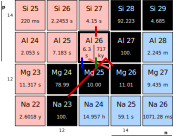
\includegraphics[width=0.5\textwidth]{graphics/solar_system_slrs/al26_chartnuc}
    \caption{Production and destruction path for the synthesis of \ex{26}Al.}
    \label{fig:solar_system_slrs:al26_production_destruction}
\end{figure}
Figure~\ref{fig:solar_system_slrs:al26_production_destruction} shows nuclear reactions that lead to the production and destruction of \ex{26}Al. Generally, \ex{26}Al is formed by proton capture on \ex{25}Mg. This can lead to \ex{26}Al that is either in the ground state, which has a half-life of $7.17\times10^{5}$\,a, or in an isomeric state with a half-life of 6.3\,s. The feeding factors are highly uncertain, which induces large uncertainties for the production and destruction factors of \ex{26}Al in stellar environments. In very proton-rich environments, \ex{26}Al in the ground state can undergo another proton capture and be destroyed via $^{26}\mathrm{Al}(p,\gamma){^{27}}\mathrm{Si}$. This rate is also not well established since it is controlled by low-energy resonances that are difficult to measure. 

Major sources for the production of \ex{26}Al are \acp{sn} and \ac{wr} stars. During the \ac{wr} phase of massive stars, \ex{26}Al is produced by proton capture and released into to galaxy due to peeling of the hydrogen-burning ashes from the convective envelope by strong winds. In \acp{sn} explosions, \ex{26}Al production occurs in the O/Ne shell. Here, destruction takes mostly place by neutron captures via $^{26}\mathrm{Al}(n,p){^{26}}\mathrm{Mg}$ and $^{26}\mathrm{Al}(n,\alpha){^{23}}\mathrm{Na}$.

\paragraph{Iron-60}

Among all \acp{slr} in the early Solar System, the abundance of \ex{60}Fe has been highly controversial in the literature. Recent findings however are finally looking promising to resolve the dispute, see Section~\ref{sec:solar_system_slrs:fe60_controversy}. Iron-60 has a half-life of 2.62\,Ma. This \ac{slr}'s main production sites are \acp{sn}.

\begin{figure}[tb]
    \centering
    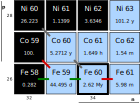
\includegraphics[width=0.4\textwidth]{graphics/solar_system_slrs/fe60_chartnuc}
    \caption{Production and destruction path for the synthesis of \ex{60}Fe.}
    \label{fig:solar_system_slrs:fe60_production_destruction}
\end{figure}
Figure~\ref{fig:solar_system_slrs:fe60_production_destruction} shows the production (green) and destruction (red) paths for \ex{60}Fe. The gray arrows indicate the radiogenic decay of \ex{60}Fe to its stable daughter \ex{60}Ni. Iron-60 is produced by two subsequent neutron captures, first on \ex{58}Fe and then on the unstable \ex{59}Fe. This latter nucleus has a half-life of 44.495\,d and can, if the $\beta^{-}$-decay to \ex{59}Co happens first, influence the amount of \ex{60}Fe that is produced. A similar branching ratio calculation as for \ex{95}Zr, see Figure~\ref{fig:s-process:branching_zr95}, can be done for \ex{60}Fe. Furthermore, in neutron-rich environment \ex{60}Fe can also capture another neutron and therefore be destroyed in the $(n,\gamma)$ reaction that produces \ex{61}Fe.

In \acp{sn}, the production of \ex{60}Fe happens via neutron capture along with the production of \ex{26}Al in the O/Ne shell during explosive nucleosynthesis. Under these conditions, enough neutron captures can take place to effectively form \ex{60}Fe. However, at hot conditions of $T_8 > 5$, the half-lives of \ex{59}Fe and \ex{60}Fe are significantly reduced, which affects the branching itself and therefore the production and survival of \ex{60}Fe.

\paragraph{Iodine-129, Plutonium-244, and Curium-247}

Iodine-129, \ex{244}Pu, and \ex{247}Cm are all \acp{slr} that are mainly produced in the \ac{rproc}, the latter two can in fact solely be produced in the \ac{rproc}. The lighter \ex{129}I is shielded in the \ac{sproc} by the short-lived \ex{128}I, which has a half-life of only 25\,min. Therefore, the branching to produce \ex{129}I cannot efficiently be activated in \ac{agb} stars.

In a recent study, \citet{cote21} used the almost identical half-lives of \ex{129}I and \ex{247}Cm of 15.7\,Ma and 15.6\,Ma, respectively, to constrain the source that contributed these nuclei to the early Solar System. Within nuclear uncertainties it seems likely that these \acp{slr} were formed and injected into the solar nebula by a single \ac{rproc} event taking place in a \ac{ns}-\ac{ns} merger. In how far \ex{244}Pu could be contributed as well in such an event is not currently known, however, comparisons of early Solar System \ex{244}Pu abundances compared to the contemporary ones \citep{wallner15} showed that this nuclide as well likely forms in rare events. 


\paragraph{Beryllium-10 (and Beryllium-7)}

The presence of \ex{10}Be (half-life $1.4\times10^{6}$\,a) in the early Solar System has long raised questions of a potential local production of these nuclei. Beryllium-10 is mainly destroyed in stars and thus cannot have a stellar origin. However, solar cosmic rays from an active early Sun or galactic cosmic rays could potentially form this nuclide in situ, i.e., via induced spallation reactions.

\begin{figure}[tb]
    \centering
    \includegraphics[width=0.8\textwidth]{graphics/solar_system_slrs/spallation}
    \caption{Schematic of a spallation reaction induced by a high energy particle. Details are described in the text.}
    \label{fig:solar_system_slrs:spallation_schematic}
\end{figure}
Figure~\ref{fig:solar_system_slrs:spallation_schematic} shows a schematic of how a spallation reaction takes place in three panels. In panel 1, a high energy proton strikes a target nucleus (here \ex{28}Si). This nucleus then breaks up into various lighter nuclei (panel 2). The excited nucleus left behind subsequently decays, e.g., via $\gamma$ or neutron emission and a cosmogenic nuclide is left behind (panel 3). In this way, \ex{10}Be can be effectively produced, e.g., from carbon, oxygen, or silicon. 

Since \ex{10}Be requires a local production scenario within the Solar System, the question poses itself how much effect such a local production would have on other \acp{slr}. Unfortunately, most models that produce \ex{10}Be in situ do not consider a real, actual irradiation scenario and often overproduce \ex{41}Ca and \ex{26}Al when producing the correct amount of \ex{10}Be. One attempt of actually simulating the production of \acp{slr} in the solar nebula showed however that it is highly difficult to irradiate dust in such a setup by cosmic rays since, since these are effectively stopped by the hydrogen gas \citep{trappitsch15}. Interestingly, this realistic production model would however result in mainly producing \ex{10}Be.

In addition to the presence of \ex{10}Be, \ex{7}Li excess from the decay of \ex{7}Be has also been detected. This \ac{slr} has a half-life of only 53\,d, making it impossible that it originated anywhere else than from a local production scenario. However, more measurements are needed to constrain if isochrons for \ex{7}Be actually exist and what types of samples contain this \ac{slr}. Clear evidence for the presence of \ex{7}Be could significantly limit the local production scenario(s) due to its short half-life.

\section{The Solar System's Birth Environment}

The timing information contained in \acp{slr} allows us to decipher the history of the Solar System just prior to its formation. Furthermore, observations of contemporary stellar nurseries can also tell us how the Solar System formation fits into the broader picture of star and planetary system formation in the Milky Way.

\subsection{Gamma-Ray Observations}

\begin{figure}[tb]
    \centering
    \includegraphics[width=\textwidth]{graphics/solar_system_slrs/al26_galaxy}
    \caption{\href{https://heasarc.gsfc.nasa.gov/docs/cgro/cgro/comptel.html}{\acs{comptel}} image of \ex{26}Al in the Milky Way. Courtesy of \href{https://www2011.mpe.mpg.de/gamma/science/lines/26Al/26Al.html}{Roland Diehl/MPE Garching}.}
    \label{fig:solar_system_slrs:comptel_al26_gamma-ray}
\end{figure}
Figure~\ref{fig:solar_system_slrs:comptel_al26_gamma-ray} shows the Milky Way imaged in $\gamma$-rays showing the decay of \ex{26}Al as imaged by the \acf{comptel}. The inset shows a spectrum taken by the \acf{integral} telescope. Clearly, \ex{26}Al is currently being produced in the Milky Way. Similar observations have also been done for \ex{60}Fe, showing the ongoing production of \acp{slr} in the Milky Way. The solar nebula was therefore not an exception and other molecular clouds also start out with a certain amount of \acp{slr}.

\subsection{Conditions}

The molecular cloud from which the Solar System formed likely formed within a giant molecular cloud from which many stars formed. Such stellar nurseries have been observed across the galaxy with various molecular clouds collapsing. Depending on their mass, these molecular clouds can form massive stars that can live fast and die young. Therefore, such events can pollute other collapsing molecular clouds with freshly produced \acp{slr}. 

\begin{figure}[tb]
    \centering
    \includegraphics[width=0.8\textwidth]{graphics/solar_system_slrs/solar_system_history}
    \caption{Schematic of the historic events that likely led to the formation of the Solar System and its \acp{slr}.}
    \label{fig:solar_system_slrs:solar_system_history}
\end{figure}
Figure~\ref{fig:solar_system_slrs:solar_system_history} shows a schematic of the historical events that likely led to the formation of the Solar System. After around 9\,Ga of \ac{gce} in the Milky Way, the giant molecular cloud from which later the Solar System formed received its last material by stellar additions. This last addition starts the clock for the isolation time $t_\mathrm{iso}$. Stars form in the giant molecular clouds, some of which are massive and therefore only have short lifetimes. These massive stars can life and die while other molecular clouds, e.g., the one that formed the System, are still collapsing. These massive stars therefore can pollute the giant molecular clouds and these forming systems with \acp{slr}. Once solids condensed in the Solar System, the radionuclide decayed in situ leading to the formation of isochrons. These isochrons can now be detected in meteoritic samples, e.g., the Allende meteorite as shown in the very right-most image in Figure~\ref{fig:solar_system_slrs:solar_system_history}.

% TODO: A GCE chapter on SLRs, see Lugaro et al. (2018b)

\subsection{The Iron-60 Controversy} \label{sec:solar_system_slrs:fe60_controversy}

Using various mineral phases and in situ measurements by \acf{sims} of meteoritic phases, the initial composition of \ex{60}Fe/\ex{56}Fe was determined by various authors to be on the order of $10^{-7}$ to $10^{-6}$ \citep[e.g.,][]{mishra14,telus18}. This ``high'' abundance would be consistent with a co-production of \ex{26}Al and \ex{60}Fe in a \ac{sn}, which could also have triggered the collapse of the Solar System's molecular cloud.

On the other hand, bulk measurements by \acf{icpms} of meteorites yielded an initial \ex{60}Fe/\ex{56}Fe ratio for the early Solar System of $(1.01 \pm 0.27)\times10^{-8}$ \citep{tang12,tang15}. This \ex{60}Fe value could easily be consistent with the galactic background. More importantly, it excludes the contribution of a \ac{sn} to the early Solar System. Since \ex{26}Al and \ex{60}Fe are both produced during explosive nucleosynthesis in the O/Ne shell, \ex{60}Fe would have to be present at ``high'' levels in order for \ex{26}Al to also have been co-injected. The almost four times longer half-life of \ex{60}Fe compared to \ex{26}Al only allows the \ex{26}Al/\ex{60}Fe ratio to decrease over time. Even within the uncertainties in the nucleosynthesis calculations, \acp{sn} would contribute too much \ex{60}Fe is supplying all \ex{26}Al \citep{jones19}. 

The two measurement methods clearly came up with mutually exclusive results for the abundance of \ex{60}Fe in the early Solar System, which resulted in a large controversy in cosmochemistry. The solution to the issue of measurement discrepancies likely originates in the data processing of the in situ measurements that determined the high \ex{60}Fe/\ex{56}Fe values. \citet{trappitsch18} re-measured one sample previously analyzed by \ac{sims} and found no effects due to in situ decay of \ex{60}Fe. Compared to the original \ac{sims} measurements, the new measurements were performed by \ac{rims}, which allows the detection of all isotopes. 

\begin{figure}[tb]
    \centering
    \includegraphics[width=\textwidth]{graphics/solar_system_slrs/fe60_int_norm}
    \caption{Simulated nickel isotope measurements, normalized to \ex{58}Ni. Left: $\delta$-values are shown along with the suspected mass-dependent fractionation (dashed, red line). Right: Measurements were internally noramlized to correct for mass-dependent fractionation.}
    \label{fig:solar_system_slrs:fe60_int_norm}
\end{figure}
Figure~\ref{fig:solar_system_slrs:fe60_int_norm} shows a simulated data set for measured nickel isotopes. The left side shows the typical $\delta$-values as defined in equation~\eqref{eqn:stardust:delta_notation} normalized to \ex{58}Ni. The red, dashed line in the background shows the effect of mass-dependent fraction, which can take place, e.g., in the instrument that is used to measure the sample. This mass-dependent fractionation can hide the actual signal, e.g., an excess in \ex{60}Ni due to in situ \ex{60}Fe decay. By assuming a solar system abundance of a second isotope along with \ex{58}Ni, the measurements can be internally normalized. This is shown on the right-hand side and generally expressed as a $\Delta$-value. Here, all simulated nickel isotopic measurements were normalized to \ex{58}Ni and \ex{62}Ni. This internal normalization is required in order to clearly detect any excess in \ex{60}Ni. Unfortunately, \ac{sims} measurements cannot determine the abundance of \ex{58}Ni due to isobaric interferences with \ex{58}Fe. Therefore, internal normalization of the measurements has to be performed using \ex{61}Ni and \ex{62}Ni. The low natural abundance of these two isotopes of 1.14\% and 3.6\%, respectively, can lead to highly correlated effects.

\begin{figure}[tb]
    \centering
    \includegraphics[width=0.6\textwidth]{graphics/solar_system_slrs/trappitsch18_fig2}
    \caption{A comparison of \ac{rims} (left) and \ac{sims} nickel isotope measurements for the same sample. \citet{trappitsch18}, \copyright\ 2018. The American Astronomical Society.}
    \label{fig:solar_system_slrs:trappitsch18_fig2}
\end{figure}
Figure~\ref{fig:solar_system_slrs:trappitsch18_fig2} shows a comparison of the \ac{rims} measurements (left) of \citet{trappitsch18} with the re-evaluated \ac{sims} measurements (right) of \citet{telus18}. Uncertainties shown in the figure were both calculated by \citet{trappitsch18} using \ac{mc} error propagation. This re-evaluation of the SIMS measurements clearly shows the correlation effects due to internal normalization with \ex{61}Ni. Since \ac{rims} allows the interference free analysis of \ex{58}Ni, \ac{rims} measurement uncertainties do not show a large correlation. Clearly, no data point shows excesses in \ex{60}Fe. Note that this figure contains no information on the elemental iron-to-nickel ratio. Therefore, excesses due to in situ decay of \ex{60}Fe would be expected to be randomly distributed here. The \ac{sims} measurements however show a highly correlated pattern. Improper propagation of uncertainties in previous work hereby led to the detection of ``high'' \ex{60}Fe in the early Solar System. An ongoing\footnote{A manuscript discussing these results in detail is currently in preparation.} re-evaluation of all \ac{sims} measurements shows that the same is true for all other \ex{60}Fe isochrons measured by \ac{sims}. This shows that presence of ``high'' \ex{60}Fe in the early Solar System has actually not been shown, which leaves the ``low'' measurement as the only detection of this \ac{slr} in meteorites. 

These new results for now solve the controversy on \ex{60}Fe in the early Solar System and require no \ac{sn} contribution of \ex{26}Al to the solar nebula, since correlated \ex{60}Fe have not been detected. This also excludes the possibility the the collapse of the molecular cloud from which the Solar System formed was triggered by a \ac{sn} shockwave. Aluminum-26 was likely contributed to the Solar System by stellar winds from a \ac{wr} star \citep{dwarkadas17}, which would explain the absence of \ex{60}Fe.


\section{Reading}
For a detailed review on the topic of \acp{slr} in the early Solar System, the reader is referred to \citet{lugaro18rad}. This extensive review also goes in-depth into stochastic \ac{gce} models and discusses the origin of the rest of the \acp{slr}. Finally, \citet{lugaro18rad} also discuss \acp{slr} within the framework of habitability, an especially interesting aspect with respect to the origin of life -- a topic that exceeds the premise of this course and requires more than just the simple synthesis of elements in stars.




